\documentclass[10pt,fleqn]{article} % Default font size and left-justified equations
\RequirePackage{UPSTI_Document}
\newcommand{\UPSTIidVersionDocument}{3}

\usepackage{longtable}
%\usepackage[%
  %  pdftitle={Contacts et mobilités},
%    pdfauthor={Geoffrey Vaquette}]{hyperref}
\usepackage{import}
\subimport{../../../../style/}{preambule.tex}
\usepackage{subcaption}

% \newcommand\bmmax{5}
% \usepackage{bm}

%\fichetrue
\fichefalse
\proffalse
%\proffalse
%\tdtrue
\tdfalse
\courstrue
%\coursfalse
\subimport{../../../../style/}{new_style}
\subimport{../../../../style/}{macros_SII}
\subimport{../../../../style/}{preambule_trou.tex}

\usepackage{siunitx}
% -------------------------------------
% Déclaration des titres
% -------------------------------------

\def\discipline{Enseignement \\Technologique \\ Transversal}
\def\xxtete{Enseignement Technologique Transversal}

\def\classe{1 STI2D}
\def\xxnumpartie{Seq 4}
\def\xxpartie{Modéliser les interactions entre solides}

\def\xxnumchapitre{Séance 1}
\def\xxchapitre{\hspace{.12cm} Modélisation des liaisons}

\def\xxposongletx{2}
\def\xxposonglettext{1.45}
\def\xxposonglety{23}
\def\xxonglet{Seq. 4 -- Se. 2}

\def\xxactivite{Cours}
\def\xxauteur{\textsl{Geoffrey Vaquette}}

\def\xxcompetences{%
\textsl{%
\textbf{Compétences visées :}
\begin{itemize}[label=\ding{112},font=\color{ocre}]
\item \textbf{CO5.1} Expliquer des éléments d’une modélisation proposée relative au comportement de tout ou partie d’un système
\item \textbf{CO5.2} Identifier des variables internes et externes utiles à une modélisation, simuler et valider le comportement du modèle
\end{itemize}
\textbf{Connaissances abordées dans ce cours : }
\begin{itemize}[label=\ding{112},font=\color{ocre}]
\item 3.1.2 Typologie des solutions constructives des liaisons entre solides
\begin{itemize}
  \item Caractérisation des liaisons sur les systèmes
\end{itemize}
\end{itemize}
%
}}

\def\xxfigures{
\begin{center}
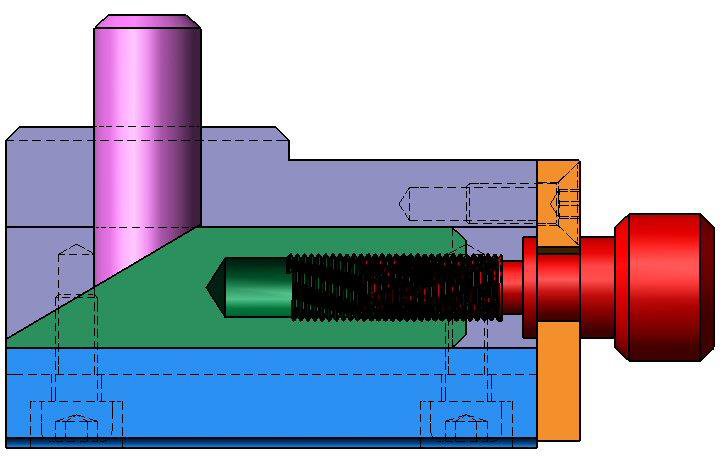
\includegraphics[width=3cm]{images/equivalence} \\
% 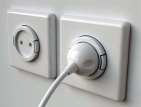
\includegraphics[width=2cm]{images/prise.png} \\
\end{center}
}%figues de la page de garde
\def\xxpied{%
La fonction alimenter/stocker \xxactivite%
}

%---------------------------------------------------------------------------

\renewcommand{\RemplirTrou}{false}


\begin{document}
\chapterimage{images/bandeau.jpg}
\subimport{../../../../style/}{new_pagegarde}
\section{Hypothèses}
\paragraph{Solides parfaits}
\begin{itemize}
    \item Géométrie parfaite.
    \begin{itemize}
        \item Solides rigides (distance entre 2 points quelconque invariante au cours du temps).
        \item Solides indéformables (forme invariable quelque soient les sollicitations imposées).
    \end{itemize}
\end{itemize}
On peut alors reconstituer la géométrie d'un solide à partir de volumes élémentaires (parallélépipède, cylindre, cône, tore, sphère).

\paragraph{Liaisons parfaites}
\begin{itemize}
    \item Pas de frottement
    \item Géométrie des contacts parfaite
\end{itemize}
Pour modéliser l'interaction entre les pièces d'un produit, la première chose à observer est le type de contacts qu'il existe entre ces pièces.

\section{Degrés de liberté et degrés de liaison}
Dès qu'il y a contact entre deux solides, il y a alors
liaison entre ces solides. Les surfaces de contact suppriment des degrés de liberté et imposent des mobilités entre les deux solides.

On peut caractériser cette liaison soit :
\begin{itemize}
    \item à partir du type de contact
    \item à partir des mouvements relatifs des pièces.
\end{itemize}

Tout mouvement  relatif  entre  solides  liés  pourra  être  obtenu  par  une  combinaison de  ces  six  mouvements  de base.

\begin{itemize}
    \item Translation suivant x (notée \trou{Tx})
    \item Translation suivant y (notée \trou{Ty})
    \item Translation suivant z (notée \trou{Tz})
    \item Rotation suivant x (notée \trou{Rx})
    \item Rotation suivant y (notée \trou{Ry})
    \item Rotation suivant z (notée \trou{Rz})
\end{itemize}


\begin{defi}
\textbf{Degrés de liaison:}
C'est le nombre de déplacements élémentaires interdits par
une liaison.

 \textbf{ Degrés  de  liberté  d'une  liaison:}

\trou{C'est  le  nombre  de  déplacements  élémentaires
indépendants autorisés par cette liaison.}

La somme des degrés de liberté et des degrés de liaison est égale à : \trou{6}.
En effet, les degrés non bloqués sont tous des degrés de liberté et inversement.
\end{defi}
\pagebreak
\begin{figure}[h]
  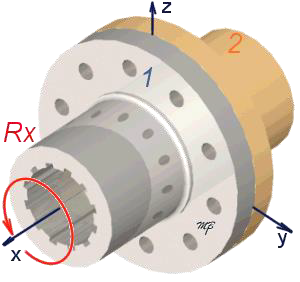
\includegraphics[width=.33\textwidth]{images/fig1} 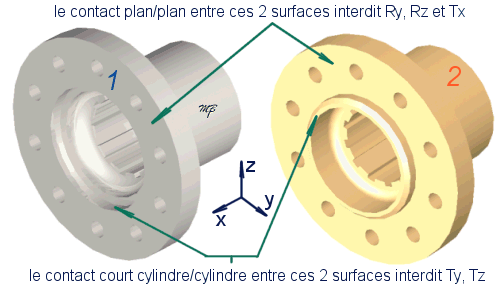
\includegraphics[width=.6\textwidth]{images/fig2}
  \caption{}
  \label{fig:plan}
\end{figure}

\begin{exemple}
  A partir de la Figure~\ref{fig:plan} et des indications, on peut déterminer les nombres de \begin{itemize}
        \item degrés de liaison : \trou{5}
        \item degrés de liberté : \trou{1}
        \item Somme : \trou{5+1=6}
  \end{itemize}
\end{exemple}
\pagebreak
\begin{footnotesize}
\begin{longtable}{>{\centering}m{2.3cm} >{\centering}m{2.6cm} >{\centering}m{2.3cm} >{\centering}m{2.2cm}>{\centering}m{2.2cm}>{\centering}p{1.9cm}} \toprule
\bf Nom & \bf Caractéristique & \bf Degrés de liberté & \bf Schéma spatial (3D)& \bf Schéma(s) plan(s) (2D)& \centering \bf Mobilités \tabularnewline
\midrule
\endhead

%------------------------------------------------------------------------------------
% Encastrement
%------------------------------------------------------------------------------------
\trou{Encastre\-ment}
&
& 0 ddl
& & &
\mobilites{0}{0}{0}{0}{0}{0}
\tabularnewline
\midrule


%------------------------------------------------------------------------------------
% Glissière
%------------------------------------------------------------------------------------
\trou{Glissière}\vspace{1em}

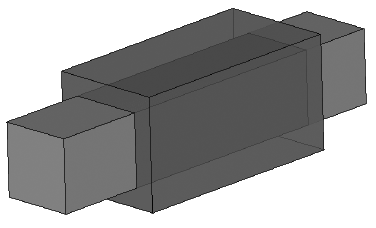
\includegraphics[width=15 mm] {Src/Images/glissiere-NB}\vspace{0.5em}
& Direction \vx{}
& 1 ddl
&
\begin{tikzpicture}[scale=0.89]
\draw [black, thick] (-0.2,0.2) -- (0.2,-0.25);
\draw [black, thick] (-0.2,-0.2) -- (0.2,0.15);
\draw [very thick] (0.9,0.35) --++(0.2,0.1) node[above, xshift=-1mm] {1};
\draw [UPSTIcustomColor1, thick] (-0.2,0.2) -- ++(0.4,-0.05) --++(0,-0.4) --++(-0.4,0.05) --++(0,0.4);
\draw [UPSTIcustomColor1, thick] (-0.2,0.2) --++(0.7,0.3) --++(0.4,-0.05) --++(-0.7,-0.3);
\draw [UPSTIcustomColor1, thick] (0.2,-0.25) --++(0.7,0.3) --++(0,0.4);
\draw [UPSTIcustomColor1, thick] (0.35,0.325) --++(0.3,0.6) node [above] {2};
\draw [UPSTIcustomColor1, fill=UPSTIcustomColor1, thick] (0.35,0.325) --++(0.07,0.03) --++(0,0.1) -- (0.35,0.325);
\draw [->,>=latex] (0.35,0.325) --++(0,1) node[left] {$\vv z$};
\draw [->,>=latex] (0.5,0.1) --++(0.6,-0.075) node[below left] {$\vv y$};
\draw [->,>=latex] (0,-0.035) --++(-0.5,-0.25) node[below] {$\vv x$};
\draw [very thick] (0,-0.035) --++(-0.2,-0.1) --++(-0.36,0.045) coordinate(A);
\draw [fill=black] (A) circle (0.05) node[above] {$M$};
\end{tikzpicture}
&
\begin{tikzpicture}[scale=0.9]
% 2D côté
\begin{scope}[xshift=0.35cm, yshift=1.5cm, scale=1]
\draw [very thick] (0.25,0) node[below] {1} -- (-1,0); 
\draw [->,>=latex] (-1.1,0) --(-1.5,0) node[above right] {$\vv x$};
\draw [fill=black] (-1,0) circle (0.05) node[below] {$M$};
\draw [UPSTIcustomColor1, fill=UPSTIcustomColor1, thick] (-0.35,0.2) --++(0.1,0) --++(0,0.1) -- (-0.35,0.2);
\draw [UPSTIcustomColor1, fill=white, thick] (-0.7,0.2) rectangle (0,-0.2);
\draw [UPSTIcustomColor1, thick] (-0.35, 0.2) --++(0.3,0.3) node[right] {2};
\draw [->,>=latex] (-0.35,0.3) --(-0.35,0.9) node[right] {$\vv z$};
\draw (-1.2,0.8) circle (0.1) node [right] {$\vv y$};
\draw [fill=black](-1.2,0.8) circle (0.02);
\draw [UPSTIcustomColor1, fill=UPSTIcustomColor1] (-0.35,0.2) --++(0.1,0) --++(0,0.1) -- (-0.35,0.2);
\end{scope}

 % 2D face
 \begin{scope}[xshift=0cm, yshift=0cm, scale=1]
\draw [black, thick] (-0.2,0.2) -- (0.2,-0.2);
\draw [black, thick] (-0.2,-0.2) -- (0.2,0.2);
\draw [UPSTIcustomColor1, thick] (-0.2,0.2) rectangle (0.2,-0.2);
\draw [UPSTIcustomColor1, thick] (0,0.2) -- (0,0.6) node[below right] {2};
\draw [very thick] (0,0) -- (-0.7,0) node[below right] {1};
\draw [fill=black] (-0.7,0) circle (0.05) node[above] {$M$};
\draw [->,>=latex] (0.25,0) --(0.7,0) node[below] {$\vv y$};
\draw [->,>=latex] (0,0.65) --(0,1) node[right] {$\vv z$};
\draw (-0.8,0.8) circle (0.1) node [right] {$\vv x$};
\draw [fill=black](-0.8,0.8) circle (0.02);
\end{scope}
\end{tikzpicture}
&
\mobilites{0}{0}{0}{1}{0}{0}
\tabularnewline
\midrule


%------------------------------------------------------------------------------------
% Pivot
%------------------------------------------------------------------------------------
\trou{Pivot}\vspace{1em}

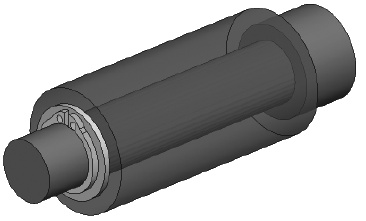
\includegraphics[width=15 mm] {Src/Images/pivot-NB}\vspace{0.5em}
& Axe \axe{A}{\vx{}}
& 1 ddl
&
\begin{tikzpicture}[scale=0.89]
\draw [very thick] (0.9,0.35) --++(0.2,0.085) node [below] {1};
\draw [very thick] (0.925,0.35) --++(0,0.2);
\draw [rotate=20, UPSTIcustomColor1, thick] (0,0) circle (0.1 and 0.2);
\draw [shift={(0.9,0.15)},rotate=20, UPSTIcustomColor1, thick, fill=white] (0,0) arc (-90:90:0.1 and 0.2);
\draw [UPSTIcustomColor1, thick] (-0.06,0.19) --++(0.84,0.34);
\draw [UPSTIcustomColor1, thick] (0.06,-0.19) --++(0.84,0.34);
\draw [UPSTIcustomColor1, thick] (0.35,0.325) --++(0.3,0.6) node [right] {2};
\draw [UPSTIcustomColor1, fill=UPSTIcustomColor1, thick] (0.35,0.325) --++(0.07,0.03) --++(0,0.1) -- (0.35,0.325);
\draw [->,>=latex] (0.35,0.325) --++(0,1) node[left] {$\vv z$};
\draw [->,>=latex] (0.5,0.1) --++(0.5,-0.2) node[below left] {$\vv y$};
\draw [->,>=latex] (0,0) --++(-0.6,-0.257) node[below right] {$\vv x$};
\draw [very thick] (0,0) --++(-0.3,-0.129) coordinate(A);
\draw [fill=black] (A) circle (0.05) node[above] {$A$};
\draw [very thick] (-0.075,0.15) --++(0,-0.35);
\end{tikzpicture}
&
\begin{tikzpicture}[scale=0.9]
% 2D côté
\begin{scope}[xshift=0.35cm, yshift=1.5cm, scale=1]
\draw [UPSTIcustomColor1, thick] (-0.7,0.2) rectangle (0,-0.2);
\draw [very thick] (0.25,0) node[below] {1} -- (-1,0); 
\draw [->,>=latex] (-1.1,0) --(-1.5,0) node[above right] {$\vv x$};
\draw [fill=black] (-1,0) circle (0.05) node[below] {$A$};
\draw [very thick] (-0.78, 0.2) --++(0,-0.4);
\draw [very thick] (0.08, 0.2) --++(0,-0.4);
\draw [UPSTIcustomColor1, fill=UPSTIcustomColor1, thick] (-0.35,0.2) --++(0.1,0) --++(0,0.1) -- (-0.35,0.2);
\draw [UPSTIcustomColor1, thick] (-0.35, 0.2) --++(0.3,0.3) node[right] {2};
\draw [->,>=latex] (-0.35,0.3) --(-0.35,0.9) node[right] {$\vv z$};
\draw (-1.2,0.8) circle (0.1) node [right] {$\vv y$};
\draw [fill=black](-1.2,0.8) circle (0.02);
\draw [UPSTIcustomColor1, fill=UPSTIcustomColor1] (-0.35,0.2) --++(0.1,0) --++(0,0.1) -- (-0.35,0.2);

\end{scope}

% 2D face
\begin{scope}[xshift=0cm, yshift=0cm, scale=1]
\draw [UPSTIcustomColor1, thick] (0,0.2) -- (0,0.6) node[below right] {2};
\draw [very thick] (0,0) -- (-0.7,0) node[below right] {1};
\draw [UPSTIcustomColor1, thick, fill=white] (0,0) circle (0.2);
\draw [UPSTIcustomColor1, fill=UPSTIcustomColor1] (0,0.3) --++(0,-0.1) arc (90:110:0.2) -- (0,0.3);
\draw [->,>=latex] (0.25,0) --(0.7,0) node[below] {$\vv y$};
\draw [->,>=latex] (0,0.65) --(0,1) node[right] {$\vv z$};
\draw (-0.8,0.8) circle (0.1) node [right] {$\vv x$};
\draw [fill=black](-0.8,0.8) circle (0.02);
\node at (0.2,-0.25) [] {$A$};
\draw [ultra thin] (-0.05,0) --++(0.1,0);
\draw [ultra thin] (0,-0.05) --++(0,0.1);
\end{scope}

\end{tikzpicture}
&
\mobilites{1}{0}{0}{0}{0}{0}
\tabularnewline
\midrule


%------------------------------------------------------------------------------------
% Hélicoïdale
%------------------------------------------------------------------------------------
\trou{Hélicoïdale}\vspace{1em}
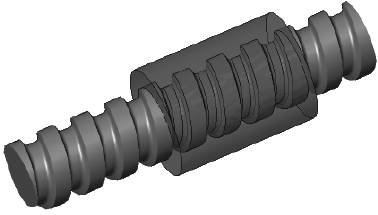
\includegraphics[width=15 mm] {Src/Images/helicoidale-NB}%\vspace{0.5em}
& Axe \axe{A}{\vx{}}
& 1 ddl
&
\begin{tikzpicture}[scale=0.89]
\draw [very thick] (0.9,0.35) --++(0.2,0.085) node [below] {1};
\draw [rotate=20, UPSTIcustomColor1, thick] (0,0) circle (0.1 and 0.2);
\draw [rotate=20, UPSTIcustomColor1, thick, fill=white, shift={(0.9,-0.17)}] (0,0) arc (-90:90:0.1 and 0.2);
\foreach \x in {0.1,0.2, ...,0.8} \draw [rotate=22, very thick, shift={(\x,-0.2)}] (0,0) arc (-90:90:0.1 and 0.2);
\draw [UPSTIcustomColor1, thick] (-0.06,0.19) --++(0.84,0.34);
\draw [UPSTIcustomColor1, thick] (0.06,-0.19) --++(0.84,0.34);
\draw [UPSTIcustomColor1, thick] (0.35,0.325) --++(0.3,0.6) node [right] {2};
\draw [UPSTIcustomColor1, fill=UPSTIcustomColor1, thick] (0.35,0.325) --++(0.07,0.03) --++(0,0.1) -- (0.35,0.325);
\draw [->,>=latex] (0.35,0.325) --++(0,1) node[left] {$\vv z$};
\draw [->,>=latex] (0.5,0.1) --++(0.5,-0.2) node[below left] {$\vv y$};
\draw [->,>=latex] (0,0) --++(-0.6,-0.257) node[below right] {$\vv x$};
\draw [very thick] (0,0) --++(-0.3,-0.129) coordinate(A);
\draw [fill=black] (A) circle (0.05) node[above] {$A$};
\end{tikzpicture}
&
\begin{tikzpicture}[scale=0.9]
% 2D côté
\begin{scope}[xshift=0.35cm, yshift=1.5cm, scale=1]
\draw [UPSTIcustomColor1, thick, fill=white] (-0.72,0.2) rectangle (0,-0.2);
\draw [very thick] (0.25,0) node[below] {1} -- (0,0); 
\draw [very thick] (-0.72,0) -- (-1,0); 
\draw [->,>=latex] (-1.1,0) --(-1.5,0) node[above right] {$\vv x$};
\draw[domain=-0.72:0,samples=80,very thick] plot ({\x},{0.1*sin(2000*\x)});
\draw [fill=black] (-1,0) circle (0.05) node[below] {$A$};
\draw [UPSTIcustomColor1, fill=UPSTIcustomColor1, thick] (-0.35,0.2) --++(0.1,0) --++(0,0.1) -- (-0.35,0.2);
\draw [UPSTIcustomColor1, thick] (-0.35, 0.2) --++(0.3,0.3) node[right] {2};
\draw [->,>=latex] (-0.35,0.3) --(-0.35,0.9) node[right] {$\vv z$};
\draw (-1.2,0.8) circle (0.1) node [right] {$\vv y$};
\draw [fill=black](-1.2,0.8) circle (0.02);
\draw [UPSTIcustomColor1, fill=UPSTIcustomColor1] (-0.35,0.2) --++(0.1,0) --++(0,0.1) -- (-0.35,0.2);
\end{scope}

 % 2D face
 \begin{scope}[xshift=0cm, yshift=0cm, scale=1]
\draw [UPSTIcustomColor1, thick] (0,0.2) -- (0,0.6) node[below right] {2};
\draw [very thick] (0,0) -- (-0.7,0) node[below right] {1};
\draw [UPSTIcustomColor1, thick, fill=white] (0,0) circle (0.2);
\draw [UPSTIcustomColor1, fill=UPSTIcustomColor1] (0,0.3) --++(0,-0.1) arc (90:110:0.2) -- (0,0.3);
\draw [->,>=latex] (0.25,0) --(0.7,0) node[below] {$\vv y$};
\draw [->,>=latex] (0,0.65) --(0,1) node[right] {$\vv z$};
\draw (-0.8,0.8) circle (0.1) node [right] {$\vv x$};
\draw [fill=black](-0.8,0.8) circle (0.02);
\node at (0.2,-0.25) [] {$A$};
\draw [very thick] (0,0.125) arc (90:-180:0.125);
\end{scope}
\end{tikzpicture}
&
\mobilites{1}{0}{0}{1}{0}{0}
\tabularnewline
\midrule


%------------------------------------------------------------------------------------
% Pivot glissant
%------------------------------------------------------------------------------------
\trou{Pivot glissant}\vspace{1em}

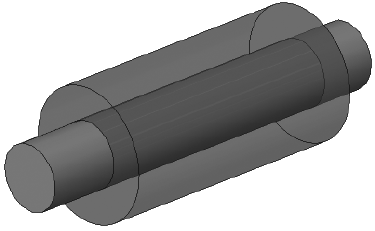
\includegraphics[width=15 mm] {Src/Images/pivot-glissant-NB}%\vspace{0.5em}
& Axe \axe{A}{\vx{}}
& 2 ddl
&
\begin{tikzpicture}[scale=0.89]
\draw [very thick] (0.93,0.37) --++(0.2,0.085) node [below] {1};
\draw [rotate=20, UPSTIcustomColor1, thick] (0,0) circle (0.1 and 0.2);
%\draw [shift={(0.9,0.15)},rotate=20, UPSTIcustomColor1, thick, fill=white] (0,0) arc (-90:90:0.1 and 0.2);
\draw [shift={(0.9,0.15)},rotate=20, UPSTIcustomColor1, thick] (0,0) arc (-90:90:0.1 and 0.2);
\draw [UPSTIcustomColor1, thick] (-0.06,0.19) --++(0.84,0.34);
\draw [UPSTIcustomColor1, thick] (0.06,-0.19) --++(0.84,0.34);
\draw [UPSTIcustomColor1, thick] (0.35,0.325) --++(0.3,0.6) node [right] {2};
\draw [UPSTIcustomColor1, fill=UPSTIcustomColor1, thick] (0.35,0.325) --++(0.07,0.03) --++(0,0.1) -- (0.35,0.325);
\draw [->,>=latex] (0.35,0.325) --++(0,1) node[left] {$\vv z$};
\draw [->,>=latex] (0.5,0.1) --++(0.5,-0.2) node[below left] {$\vv y$};
\draw [->,>=latex] (0,0) --++(-0.6,-0.257) node[below right] {$\vv x$};
\draw [very thick] (0,0) --++(-0.3,-0.129) coordinate(A);
\draw [fill=black] (A) circle (0.05) node[above] {$A$};
\end{tikzpicture}
&
\begin{tikzpicture}[scale=0.9]
% 2D côté
\begin{scope}[xshift=0.35cm, yshift=1.5cm, scale=1]
\draw [UPSTIcustomColor1, thick] (-0.7,0.2) rectangle (0,-0.2);
\draw [very thick] (0.25,0) node[below] {1} -- (-1,0); 
\draw [->,>=latex] (-1.1,0) --(-1.5,0) node[above right] {$\vv x$};
\draw [fill=black] (-1,0) circle (0.05) node[below] {$A$};
\draw [UPSTIcustomColor1, fill=UPSTIcustomColor1, thick] (-0.35,0.2) --++(0.1,0) --++(0,0.1) -- (-0.35,0.2);
\draw [UPSTIcustomColor1, thick] (-0.35, 0.2) --++(0.3,0.3) node[right] {2};
\draw [->,>=latex] (-0.35,0.3) --(-0.35,0.9) node[right] {$\vv z$};
\draw (-1.2,0.8) circle (0.1) node [right] {$\vv y$};
\draw [fill=black](-1.2,0.8) circle (0.02);
\draw [UPSTIcustomColor1, fill=UPSTIcustomColor1] (-0.35,0.2) --++(0.1,0) --++(0,0.1) -- (-0.35,0.2);
\end{scope}

 % 2D face
\begin{scope}[xshift=0cm, yshift=0cm, scale=1]
\draw [UPSTIcustomColor1, thick] (0,0.2) -- (0,0.6) node[below right] {2};
\draw [very thick] (-0.2,0) -- (-0.7,0) node[below right] {1};
%\draw [UPSTIcustomColor1, thick, fill=white] (0,0) circle (0.2);
\draw [UPSTIcustomColor1, thick] (0,0) circle (0.2);
\draw [UPSTIcustomColor1, fill=UPSTIcustomColor1] (0,0.3) --++(0,-0.1) arc (90:110:0.2) -- (0,0.3);
\draw [->,>=latex] (0.25,0) --(0.7,0) node[below] {$\vv y$};
\draw [->,>=latex] (0,0.65) --(0,1) node[right] {$\vv z$};
\draw (-0.8,0.8) circle (0.1) node [right] {$\vv x$};
\draw [fill=black](-0.8,0.8) circle (0.02);
\draw [fill=black](0,0) circle (0.04);
\node at (0.2,-0.25) [] {$A$};
\end{scope}
\end{tikzpicture}
&
\mobilites{1}{0}{0}{1}{0}{0}
\tabularnewline
\midrule


%------------------------------------------------------------------------------------
% Appui plan
%------------------------------------------------------------------------------------
\trou{Appui plan}\vspace{1em}

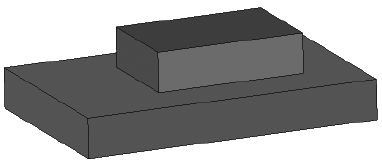
\includegraphics[width=15 mm] {Src/Images/appui-plan-NB}\vspace{0.5em}
& Normale au plan $ \vz{}$
& 3 ddl
&
\begin{tikzpicture}[scale=0.8]
\draw [thick, UPSTIcustomColor1] (0.45,-0.3) --++(0.5,-0.5) node[left] {2};
\draw [UPSTIcustomColor1, thick, fill=white] (-0.5,-0.5) --++(1,0) --++(0.75,0.25) --++(-1,0) --++(-0.75,-0.25);
\draw [fill=white, thick] (-0.5,-0.4) --++(1,0) --++(0.75,0.25) --++(-1,0) --++(-0.75,-0.25);
\draw [thick] (0.45,-0.25) --++(-0.5,0.5) node[left] {1};
\draw [->,>=latex] (0.45, -0.325) --++(1,0) node[below left] {$\vv y$};
\draw [->,>=latex] (0.45, -0.325) --++(0,1) node[above] {$\vv z$};
\draw [->,>=latex] (0.45, -0.325) --++(-0.9,-0.3) node[below right] {$\vv x$};
\draw [fill=black] (0.45,-0.25) --++(-0.1,-0.033) --++(0,0.1) -- (0.45,-0.25);
\draw [fill=black] (1,0.5) circle (0.025) node[above] {$M$};
\end{tikzpicture}
&
\begin{tikzpicture}[scale=0.9]
\draw [UPSTIcustomColor1, thick] (-0.5,-0.05) --++(1,0);
\draw [thick] (-0.5,0.05) --++(1,0);
\draw [UPSTIcustomColor1, thick] (0,-0.05) --++(0.5,-0.5) node [right] {2};
\draw [thick] (0,0.05) --++(-0.5,0.5) node [left] {1};
\draw [UPSTIcustomColor1, fill=UPSTIcustomColor1] (0,-0.05) --++(0.1,0) --++(0,-0.1) --(0,-0.05);
\draw [fill=black] (0,0.05) --++(-0.1,0) --++(0,0.1) --(0,0.05);
\draw [->, >=latex] (0,0) --++(0.75,0) node[above] {$\vv y$};
\draw [->, >=latex] (0,0) --++(0,0.75) node[left] {$\vv z$};
\draw (-0.5,-0.5) circle (0.1) node[right] {$\vv x$};
\draw [fill=black] (-0.5,-0.5) circle (0.02);
\draw [fill=black] (0.35,0.5) circle (0.025) node[above] {$M$};
\end{tikzpicture}
&
\mobilites{0}{0}{1}{1}{1}{0}
\tabularnewline
\midrule

%------------------------------------------------------------------------------------
% Sphérique
%------------------------------------------------------------------------------------
\trou{Sphérique}\vspace{1em}

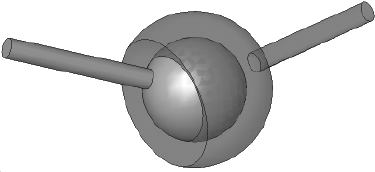
\includegraphics[width=15 mm] {Src/Images/spherique-NB}\vspace{0.5em}
& Centre de la sphère $A$
& 3 ddl
&
\begin{tikzpicture}[scale=0.89]
\draw [thick] (0,0) circle (0.2);
\draw [rotate=20, thick] (0.2,0) --++(0.6,0) node[above] {1};
\draw [UPSTIcustomColor1, very thick] (75:0.3) arc (75:330:0.3);
\draw [UPSTIcustomColor1, rotate=40, very thick] (0,0.3) --++(0,1) node[right] {2};
\node at (0.22,0.3) {$A$};
\draw [->,>=latex] (0,0) --++(0.7,-0.2) node[below] {$\vv y$};
\draw [->,>=latex] (0,0) --++(0,1.1) node[right] {$\vv z$};
\draw [->,>=latex] (0,0) --++(-0.7,-0.3) node[below] {$\vv x$};
\end{tikzpicture}
&
\begin{tikzpicture}[scale=0.9]
\draw [thick] (0,0) circle (0.2);
\draw [rotate=20, thick] (0.2,0) --++(0.6,0) node[above] {1};
\draw [UPSTIcustomColor1, very thick] (75:0.3) arc (75:330:0.3);
\draw [UPSTIcustomColor1, rotate=40, very thick] (0,0.3) --++(0,1) node[right] {2};
\node at (0.22,0.3) {$A$};
\draw [->,>=latex] (0.3,0) --++(0.7,0) node[below left] {$\vv y$};
\draw [->,>=latex] (0,0.35) --++(0,0.8) node[right] {$\vv z$};
\draw (-0.8,-0.4) circle (0.1) node [right] {$\vv x$};
\draw [fill=black] (-0.8,-0.4) circle (0.02);
\end{tikzpicture}
&
\mobilites{1}{1}{1}{0}{0}{0}
\tabularnewline
\midrule

%------------------------------------------------------------------------------------
% Sphère cylindre
%------------------------------------------------------------------------------------
\trou{Sphère cylindre}\vspace{1em}

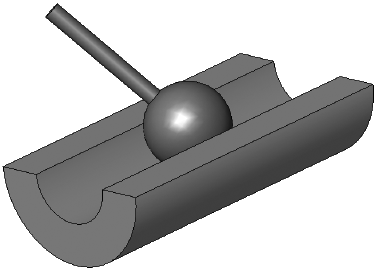
\includegraphics[width=15 mm] {Src/Images/sphere-cylindre-NB}%\vspace{0.5em}
& Centre de la sphère $A$

Direction $\vx{}$
& 4 ddl
&
\begin{tikzpicture}[scale=0.89]
\draw [thick, UPSTIcustomColor1, rotate=-20] (0,0) arc (180:360:0.2);
\draw [thick, UPSTIcustomColor1, shift={(0,0)}, rotate=19] (0,0) --++(0.8,0);
\draw [very thick] (0.5,0) --++(-0.15,0.75) node[left, xshift=1mm] {1};
\draw [very thick, fill=white] (0.675,-0.029) arc (-5:225:0.17);
\draw [thick, UPSTIcustomColor1, shift={(0.37,-0.15)}, rotate=19] (0,0) --++(0.8,0);
\draw [thick, UPSTIcustomColor1, shift={(0.25,-0.26)}, rotate=19] (0,0) --++(0.8,0);
\draw [thick, UPSTIcustomColor1, shift={(0.75,0.25)}, rotate=-20] (0,0) arc (180:260:0.2);
\draw [thick, UPSTIcustomColor1, shift={(1,0)}, rotate=-20] (0,0) arc (310:360:0.2);
\draw [thick, UPSTIcustomColor1] (0.5,-0.17) --++(0,-0.5) node[above left] {2};
\draw [->,>=latex] (0.5,0) --++(0,1) node[right] {$\vv z$};
\draw [->,>=latex] (0.5,0) --++(200:1) node[below right] {$\vv x$};
\draw [->,>=latex] (0.5,0) --++(-20:0.75) node[below left] {$\vv y$};
\node at (0.15,0.25) {$A$};
\end{tikzpicture}
&
\begin{tikzpicture}[scale=0.9]
% 2D côté
\begin{scope}[xshift=0cm, yshift=1.7cm, scale=1]
\draw [thick, UPSTIcustomColor1] (-0.28,-0.045) -- (0.28,-0.045);
\draw [thick, UPSTIcustomColor1] (0,-0.01) -- (0,-0.5) node[above right] {2};
\draw [thick, UPSTIcustomColor1] (-0.28,0.25) arc (180:360:0.28);
\draw [very thick] (0,0.25) --++(0.5,0.5) node[right] {1};
\draw [very thick, fill=white] (0,0.25) circle (0.2);
\draw [->,>=latex] (0,0.25) --++(1,0) node[below] {$\vv y$};
\draw [->,>=latex] (0,0.25) --++(0,0.9) node[left] {$\vv z$};
\node at (-0.3,0.5) {$A$};
\draw (0.5,1.25) circle (0.1) node[right] {$\vv x$};
\draw [fill=black] (0.5,1.25) circle (0.02);
\end{scope}

% 2D face
\begin{scope}[xshift=0cm, yshift=0cm, scale=1]

\draw [thick, UPSTIcustomColor1] (-0.5,0.25) rectangle (0.5,0);
\draw [thick, UPSTIcustomColor1] (0,0) -- (0,-0.5) node[above right] {2};
\draw [very thick] (0,0.25) --++(0.25,0.5) node[right] {1};
\draw [very thick, fill=white] (0,0.25) circle (0.2);
\draw [->,>=latex] (0,0.25) --++(-1,0) node[below right] {$\vv x$};
\draw [->,>=latex] (0,0.25) --++(0,0.8) node[left] {$\vv z$};
\node at (-0.3,0.5) {$A$};
\draw (-1,0.75) circle (0.1) node[right] {$\vv y$};
\draw [fill=black] (-1,0.75) circle (0.02);
\end{scope}

\end{tikzpicture}
&
\mobilites{1}{1}{1}{1}{0}{0}
\tabularnewline
\midrule


%------------------------------------------------------------------------------------
% Sphère plan
%------------------------------------------------------------------------------------
\trou{Sphère plan}\vspace{1em}

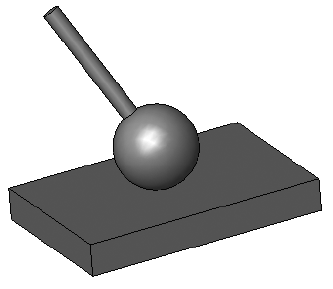
\includegraphics[width=15 mm] {Src/Images/sphere-plan-NB}\vspace{0.5em}
& Point de contact $A$

Normale au plan $\vz{}$
& 5 ddl
&
\begin{tikzpicture}[scale=0.89]
\draw [thick, UPSTIcustomColor1] (0.45,-0.3) --++(0,-0.75) node[above right] {2};
\draw [UPSTIcustomColor1, thick, fill=white] (-0.5,-0.5) --++(1,0) --++(0.75,0.5) --++(-1,0) --++(-0.75,-0.5);
\draw [very thick] (0.35,-0.15) --++(0.5,0.75) node[right] {1};
\draw [very thick, fill=white] (0.35,-0.15) circle (0.2);
\draw [->,>=latex] (0.35, -0.15) --++(0.7,-0.1) node[below] {$\vv y$};
\draw [->,>=latex] (0.35, -0.15) --++(0,1) node[right] {$\vv z$};
\draw [->,>=latex] (0.35, -0.15) --++(-0.6,-0.4) node[below] {$\vv x$};
\node at (0.15,-0.05) [above] {$A$};
\end{tikzpicture}
&
\begin{tikzpicture}[scale=0.9]
\draw [very thick, shift={(0,0.25)}, rotate=70] (0,0) --++(1,0) node[right] {1};
\draw [UPSTIcustomColor1, thick] (-0.5,-0.025) --++(1,0);
\draw [UPSTIcustomColor1, thick] (0,-0.025) --++(0.25,-0.5) node[right] {2};
\draw [very thick, fill = white] (0,0.25) circle (0.25);
\draw [->, >=latex] (0.3,0.25) --++(0.5,0) node[above] {$\vv y$};
\draw [->, >=latex] (0,0.55) --++(0,0.5) node[left] {$\vv z$};
\draw (-0.5,-0.5) circle (0.1) node[above] {$\vv x$};
\draw [fill=black] (-0.5,-0.5) circle (0.02);
\node at (-0.4,0.4) [] {$A$};
\draw [thin] (-0.05,0.25) --++(0.1,0);
\draw [thin] (0,0.2) --++(0,0.1);
\end{tikzpicture}
&\mobilites{1}{1}{1}{1}{1}{0}
\tabularnewline
\midrule


%------------------------------------------------------------------------------------
% Sphérique à doigt
%------------------------------------------------------------------------------------
\trou{Sphérique à doigt}\vspace{1em}

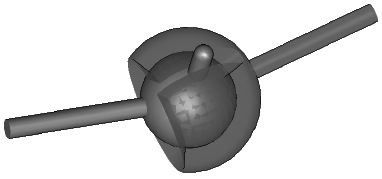
\includegraphics[width=15 mm] {Src/Images/spherique-doigt-NB}\vspace{0.5em}
& Centre de la sphère $A$

Normale au plan $\vx{}$

Direction du doigt $\vz{}$
& 2 ddl
&
\begin{tikzpicture}[scale=0.89]
\draw [thick] (0,0) circle (0.2);
\draw [rotate=20, thick] (0.2,0) --++(0.6,0) node[above] {1};
\draw [UPSTIcustomColor1, very thick] (75:0.3) arc (75:330:0.3);
\draw [UPSTIcustomColor1, rotate=40, very thick] (0,0.3) --++(0,1) node[right] {2};
\node at (0.22,0.3) {$A$};
\draw [ultra thick] (0,0.2) -- (0,0.5);
\draw [->,>=latex] (0,0) --++(0.7,-0.2) node[below] {$\vv y$};
\draw [->,>=latex] (0,0) --++(0,1.1) node[right] {$\vv z$};
\draw [->,>=latex] (0,0) --++(-0.7,-0.3) node[below] {$\vv x$};
\end{tikzpicture}
&
\begin{tikzpicture}[scale=0.9]
\draw [thick, fill=white] (0,0) circle (0.2);
\draw [rotate=20, thick] (0.2,0) --++(0.6,0) node[above] {1};
\draw [UPSTIcustomColor1, very thick] (75:0.3) arc (75:330:0.3);
\draw [ultra thick] (0,0.2) -- (0,0.5);
\draw [UPSTIcustomColor1, rotate=40, very thick] (0,0.3) --++(0,1) node[right] {2};
\node at (0.22,0.3) {$A$};
\draw [->,>=latex] (0.3,0) --++(0.7,0) node[below left] {$\vv y$};
\draw [->,>=latex] (0,0.55) --++(0,0.5) node[right] {$\vv z$};
\draw (-0.8,-0.4) circle (0.1) node [right] {$\vv x$};
\draw [fill=black] (-0.8,-0.4) circle (0.02);
\end{tikzpicture}
&
\mobilites{1}{0}{1}{0}{0}{0}
\tabularnewline
\midrule


%------------------------------------------------------------------------------------
% Linéaire rectiligne
%------------------------------------------------------------------------------------
\trou{Linéaire rectiligne} (ou cylindre plan)\vspace{1em}

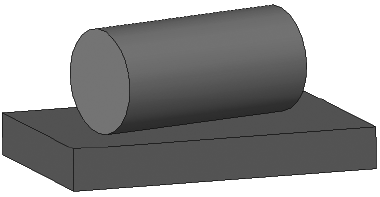
\includegraphics[width=15 mm] {Src/Images/lineaire-rectiligne-NB}\vspace{0.5em}
& Droite de contact \axe{A}{\vx{}}

Normale au plan \vz{}
& 4 ddl
&
\begin{tikzpicture}[scale=0.89]
\draw [thick, UPSTIcustomColor1] (0.45,-0.3) --++(0,-0.75) node[above right] {2};
\draw [UPSTIcustomColor1, thick, fill=white] (-0.5,-0.5) --++(1,0) --++(0.75,0.5) --++(-1,0) --++(-0.75,-0.5);
\draw [very thick, fill=white] (0.25,-0.35) --++(-0.15,0.35) --++(0.3, 0) --++(0.45,0.3) --++(-0.15,-0.35) --++(-0.45,-0.3) --++(0.15,0.35);
\draw [very thick] (0.08,0) --++(0.48,0.32) --++(0.3,0);
\draw [->,>=latex] (0.25,-0.35) --++(-0.6,-0.4) node[below, xshift=1mm] {$\vv x$};
\draw [->,>=latex] (0.46,-0.21) --++(0.75,0) node[below,xshift=-1.5mm] {$\vv y$};
\draw [->,>=latex] (0.46,-0.21) --++(0,1.2) node[left] {$\vv z$};
\draw [very thick] (0.46,0.1) --++(0.25,0.75) node[right] {1};
\node at (0.46,-0.21) [below, yshift=0.7mm] {$A$};
\end{tikzpicture}
&
\begin{tikzpicture}[scale=0.89]
% 2D côté
\begin{scope}[xshift=0cm, yshift=1.7cm, scale=1]
\draw [UPSTIcustomColor1, thick] (-0.25,0) --++(0.5,0);
\draw [UPSTIcustomColor1, thick] (0,0) --++(0,-0.4) node[left] {2};
\draw [very thick] (0,0) -- (0.15,0.35) -- (-0.15,0.35) -- (0,0);
\draw [ultra thick] (0,0.35) --++(0,0.5) node[below left, xshift=1mm] {1}; 
\draw [->, >=latex] (0.35,0) --++(0.4,0) node[below] {$\vv y$};
\draw [->, >=latex] (0,0.65) --++(0,0.5) node[left] {$\vv z$};
\draw (0.5,0.75) circle (0.1) node[above] {$\vv x$};
\draw [fill=black] (0.5,0.75) circle (0.02);
\node at (0,0) [shift={(0.15,-0.15)}] {$A$};
\end{scope}

% 2D face
\begin{scope}[xshift=0cm, yshift=0cm, scale=1]
\draw [UPSTIcustomColor1, thick] (-0.5,0) --++(1,0);
\draw [UPSTIcustomColor1, thick] (0,0) --++(0,-0.5) node[left] {2};
\draw [very thick] (-0.25,0.025) --++(0.5,0) --++(0.1,0.35) --++(-0.7,0) --cycle;
\draw [->, >=latex] (-0.55,0) --++(-0.45,0) node[above] {$\vv x$};
\draw [->, >=latex] (0,0.4) --++(0,0.7) node[left,yshift=-3mm] {$\vv z$};
\draw (-1,-0.5) circle (0.1) node[right] {$\vv y$};
\draw [fill=black] (-1,-0.5) circle (0.02);
\draw [very thick] (0,0.37) --++(0.25,0.5) node[right] {1};
\node at (0,0) [shift={(0.15,-0.15)}] {$A$};
\draw [fill=black] (0,0.37) --++(0.1,0) --++(0,0.2) --cycle;
\end{scope}
\end{tikzpicture}
&
\mobilites{1}{0}{1}{1}{1}{0}
\tabularnewline
\bottomrule

\caption{Tableau des liaisons normalisées}
\label{Cinemat_cours_tabliaison}
\end{longtable}
\end{footnotesize}

\section{Schématisation cinématique}
Une classe d’équivalence est un groupe de pièces n’ayant aucun \trou{degré de liberté} (ou aucun mouvement relatif) entre elles. On dit aussi sous-ensemble cinématiquement lié.
La recherche des classes d'équivalence passe par la localisation de toutes les liaisons encastrement (liaisons complètes) réalisées à l'intérieur du mécanisme pour la phase de fonctionnement étudiée.

\section{Graph des liaisons}
Le graphe des liaisons est un graphe utilisé pour décrire les \trou{liaisons} entre les éléments ou pièces d'un dispositif, mécanisme ou système.Le graphe se compose de cercles (ou ellipses) dans lesquels sont inscrits les noms ou les repères des composants du système étudié.
À chaque fois qu'il existe un lien ou une liaison entre deux classes d’équivalence, les cercles correspondants sont reliés l'un à l'autre par un trait et la nature de la liaison est indiquée à proximité (pivot...).

\begin{figure}[!ht]
\centering
\begin{grapheLiaisons}[scale=0.45]
\glBati{1,0.5}{P0}{0}[1/0.45]
\glPiece{4,5}{P1}{1}
\glPiece{10,2}{P2}{2}
\glLiaison[bend left]{P0}{P1}[Sphère cylindre\\ axe \axe{C}{\vx{}}][above=0.8em,left]
\glLiaison[bend right]{P0}{P1}[Sphérique\\ centre $B$][right=0.5em]
\glLiaison[bend left]{P1}{P2}[Sphère plan\\ normale \axe{D}{\vx2}][above=0.8em,right]
\glLiaison[bend left]{P2}{P0}[Pivot axe \axe{A}{\vz{}}][below]
\end{grapheLiaisons}
\caption{Exemple de graphe de liaisons d'un mécanisme}
\label{graphe_liaisons_ex}
\end{figure}

\begin{warn} Attention :
  \begin{itemize}
  \item une liaison existe chaque fois que deux classes d'équivalence ont des surfaces directement en contact ;
  \item on fait toujours l'hypothèse que les liaisons sont géométriquement parfaites ;
  \end{itemize}
\end{warn}

\section{Schéma cinématique}

À chaque liaison est associé un symbole normalisé, en fonction du plan de représentation du schéma, il suffit de placer chaque symbole au point de liaison en respectant l'orientation et le contenant / contenu.

On relie, ensuite chaque classe d'équivalence par des segments, en essayant de respecter la forme globale des groupes de pièces.

\begin{figure}[h]
  \centering
  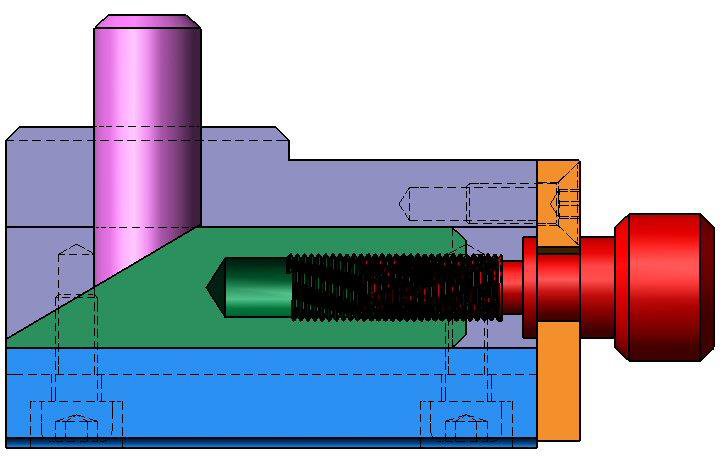
\includegraphics[width=0.4\textwidth]{images/equivalence}
  \caption{Système}
  \label{}
\end{figure}

Sur la figure~\ref{fig:complete}, dessiner les liaisons afin de parvenir au schéma cinématique.
\begin{figure}[h]
  \centering
  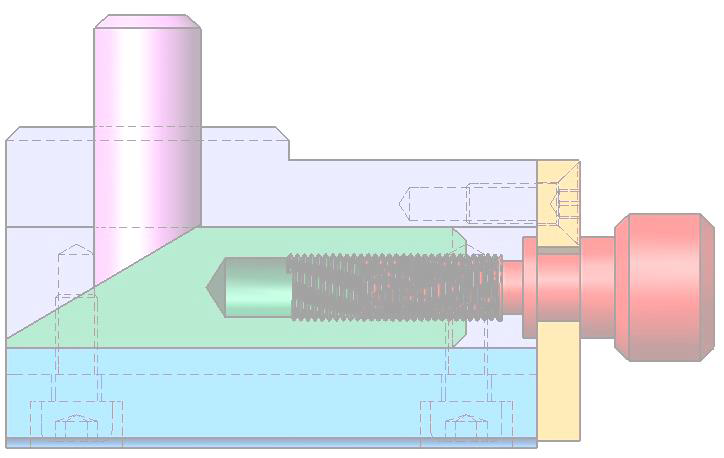
\includegraphics[width=0.4\textwidth]{images/equivalence_transparent}
  \caption{A compéter avec le schéma cinématique}
  \label{fig:complete}
\end{figure}

\begin{figure}
  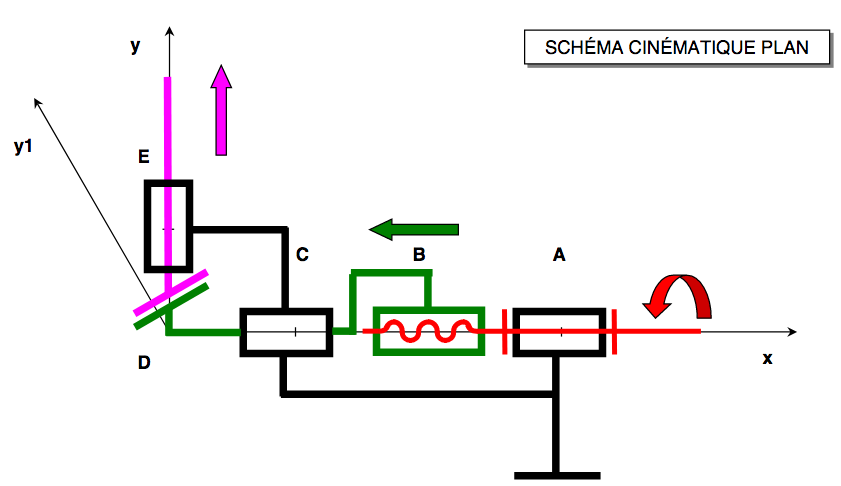
\includegraphics[width=\textwidth]{images/schema_plan}
  \caption{Schéma cinématique plan}
  \label{}
\end{figure}

\begin{figure}
  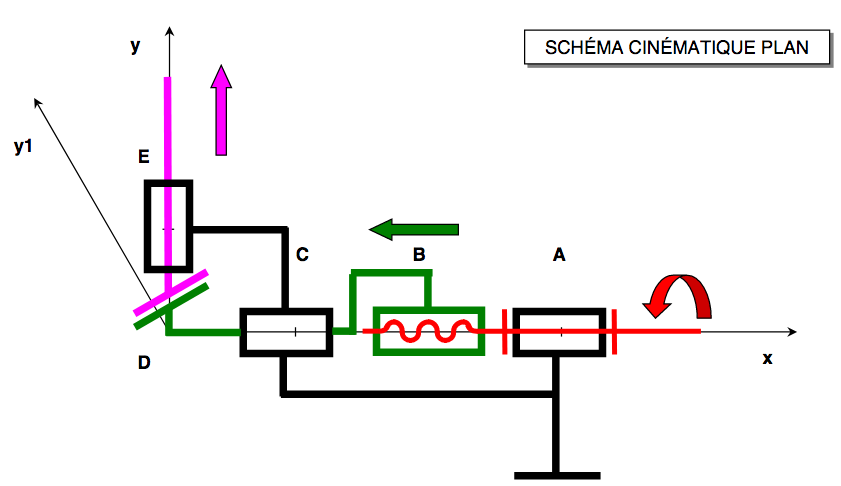
\includegraphics[width=\textwidth]{images/schema_plan}
  \caption{Schéma cinématique spatial}
  \label{}
\end{figure}
\end{document}
